\documentclass{article}
\usepackage[utf8]{inputenc}

\title{Assignment 3: Minimax}
\author{Brian Jacobel}
\date{Artificial Intelligence, Fall 2013}

\usepackage{natbib}
\usepackage{graphicx}
\usepackage[margin=1in]{geometry}
\usepackage{setspace}
\usepackage{indentfirst}

\begin{document}

\maketitle

\begin{doublespace}

\section{Results}
In this lab, the minimax algorithm was implemented to play Connect-4 against a human opponent. Two variants of the algorithm were implemented: the base version of minimax, and minimax with $\alpha$-$\beta$ pruning. For each variant, ten games were played against the algorithmic opponent at each of eight ``difficulty levels" (corresponding to maximum depths in the search tree). In each game, the total number of moves considered and the time required to generate and evaluate those moves was each tallied. These two metrics for the speed of the algorithm were averaged over the ten games played at each level. The results generated from this process are graphed below.

\begin{figure}[ht!]
\centering
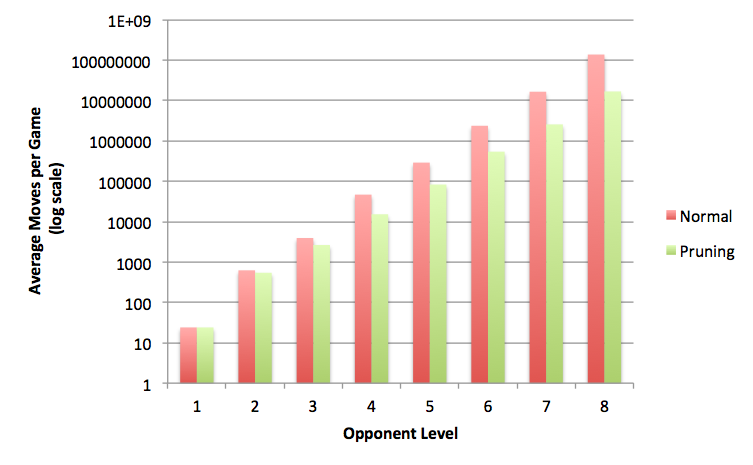
\includegraphics[width=6.5in]{../Data/Graphs/Graph2}
\caption{The average number of moves per game with pruning enabled and disabled at each of the eight opponent difficulty levels.}
\end{figure}

\begin{figure}[ht!]
\centering
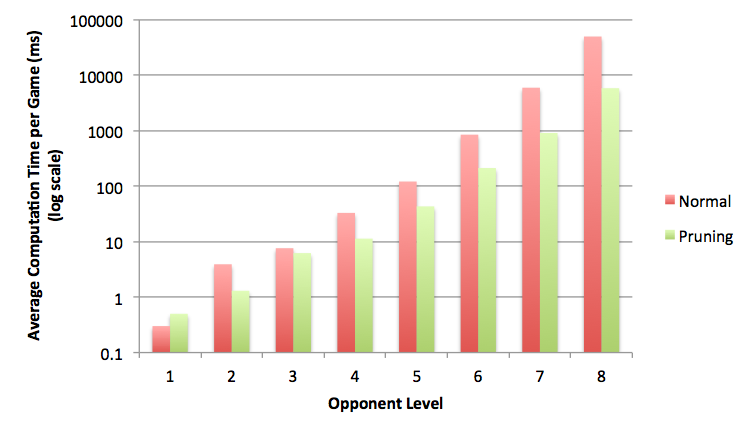
\includegraphics[width=6.5in]{../Data/Graphs/Graph3}
\caption{The average time spent exploring moves for the AI player per game with pruning enabled and disabled at each of the eight opponent difficulty levels.}
\end{figure}

As the graphs show, enabling $\alpha$-$\beta$ pruning for the algorithmic opponent reduced both the number of moves considered and the time to select the best move, at nearly all difficult levels. The extent to which $\alpha$-$\beta$ pruning affects the speed of the computer player can be better seen when expressed as percentage improvements, as in \textit{fig. 3}. As the figure shows, enabling $\alpha$-$\beta$ pruning has a large positive effect on the number of moves considered and the speed of the computer player. While results for level 3 and below are not entirely consistent, at level 4, enabling $\alpha$-$\beta$ pruning leads to a greater than 60\% improvement in both metrics of speed, and this figure increases as the limit on tree search depth is increased. Results for games played at level 3 and below likely are not as consistent because their values are comparatively small anyway, so small differences in moves inspected or CPU time would have lead to large percentage changes. Generally, these results allow us to say with great confidence that $\alpha$-$\beta$ pruning is a desirable enhancement to minimax, as it improves both the number of moves considered and the time taken before the best move is selected.

\newpage

\begin{figure}[ht!]
\centering
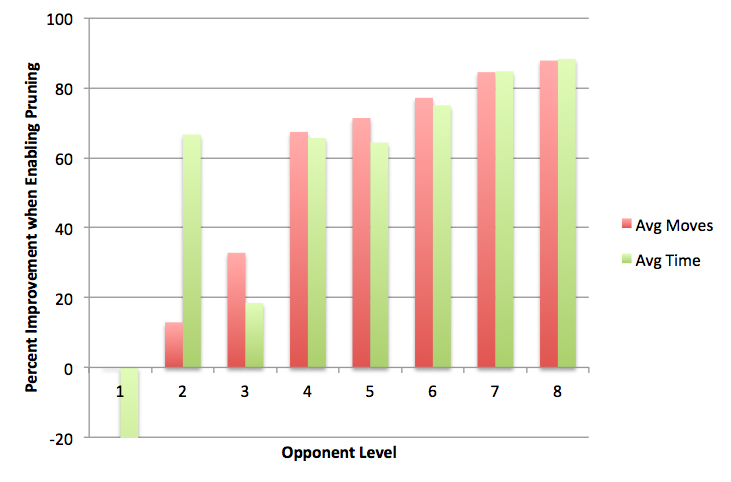
\includegraphics[width=6.5in]{../Data/Graphs/Graph1}
\caption{The effects on both the average number of moves and the average time when pruning is enabled, as compared to games at the same level with pruning disabled.}
\end{figure}

\section{Discussion}

\subsection{Heuristics}
The heuristic function analyzes game states and determines the number of 1-in-a-row, 2-in-a-row, 3-in-a-row and 4-in-a-row token positions a player has in that state. These four values are weighted together to make a "score." The number of one-in-a-row positions is weighted as one. The number of two-in-a-row positions is bit-shifted two bits to the left, which is equivalent to weighting each with four points. Likewise, the number of three-in-a-row positions in bit-shifted 5 bits, which is equivalent to weighting each as $2^5$, or 32. The number of four-in-a-row positions is weighted with the maximum score value, because this would mean the player has found a way to win.

\subsection{Ordering}
Without $\alpha$-$\beta$ pruning, the order of which rows are explored first does not matter. This is because minimax without $\alpha$-$\beta$ pruning is a complete depth-first search -- it is guaranteed to visit all nodes, and the values found at those nodes do not inform the order or choice to explore other nodes at all. With $\alpha$-$\beta$ pruning, however, doing things out of order would not be a rigorous implementation of the algorithm. Minimax with $\alpha$-$\beta$ pruning is not a complete DFS - it picks portions of the tree not to visit based on results obtained from other parts of the tree. If the tree was processed in a different order, it is possible (and likely) that different ``early returns" would be found, and different parts of the tree would not be explored. Because we want two people with the same data and the same algorithm to get the same answer, minimax with $\alpha$-$\beta$ pruning mandates a left-to-right order. We might explore nodes out of order, and might even get better results because of it, but we wouldn't be adhering to the rules of the algorithm we were supposed to implement.

\subsection{Columns}
If the program were to be modified to use 7 columns rather than 8, the unnamed constant on line 94 of \texttt{C4board.java} would need to be changed to reflect the new number of unique four-in-a-row token layouts that would exist on the smaller board. This new value would be 15 less than the previous value, because 15 "four slots" use the eighth column currently (three with $45^{\circ}$ slope, three with $-45^{\circ}$ slope, six with $0^{\circ}$ slope, and three with $90^{\circ}/-90^{\circ}$ slope). Thus the new value would be 69. It would be nice if this constant were named, yes -- I would name it something like \texttt{MAX\_WINNING\_PLAYS}.


\end{doublespace}

\end{document}



